%
% JFFS3 design issues.
%
% Copyright (C) 2005 Artem B. Bityuckiy, dedekind@infradead.org
%
% $Id: JFFS3design.tex,v 1.24 2005/11/03 14:25:39 dedekind Exp $
%

% gqap - rewrap a paragraph in vim

\documentclass[12pt,a4paper,oneside,titlepage]{article}
\usepackage{hyperref}
\usepackage{html}
\usepackage{amssymb}
\usepackage{longtable}

\begin{htmlonly}
\usepackage{graphicx}
\end{htmlonly}
%begin{latexonly}
\ifx \pdfoutput \undefined
\usepackage{graphicx}
\else
\pdfpagewidth=210mm
\pdfpageheight=297mm
\usepackage[pdftex]{graphicx}
\fi
%end{latexonly}

% Set pages layout.
% A4 paper has 210mm x 297mm
% TeX automatically makes 25.4mm left and top indents
\oddsidemargin=0mm  % 25.4mm by default
\textwidth=159.2mm  % 25.4mm right indent
\topmargin=0mm      % 25.4mm by default
\textheight=241.6mm % 30mm bottom indent
\headheight=0mm
\headsep=0mm

% Define TODO command
\newcommand{\TODO}[1]{[{\textbf{TODO}: #1}]\marginpar{\large \textbf{?!}}}

\begin{document}

%%%%%%%%%%%%%%%%%%%%%%%%%%%%%%%%%%%%%%%%%%%%%%%%%%%%%%%%%%%%%%%%%%%%%%%%%%%%%%%%
%
%  TITLE PAGE
%
%%%%%%%%%%%%%%%%%%%%%%%%%%%%%%%%%%%%%%%%%%%%%%%%%%%%%%%%%%%%%%%%%%%%%%%%%%%%%%%%
%\title{JFFS3 design issues}
%\author{Artem B. Bityuckiy}
\begin{titlepage}
\vspace*{5cm}
\begin{center}
\Huge{\textbf{JFFS3 design issues}}\\
\vspace{1cm}
\large{Artem B. Bityuckiy\\
dedekind@infradead.org}\\
\vspace{13cm}
\large{Version 0.27 (draft)}\\
\vspace{0.5cm}
November 3, 2005
\end{center}
\end{titlepage}
%\maketitle

%%%%%%%%%%%%%%%%%%%%%%%%%%%%%%%%%%%%%%%%%%%%%%%%%%%%%%%%%%%%%%%%%%%%%%%%%%%%%%%%
%
% ABSTRACT
%
%%%%%%%%%%%%%%%%%%%%%%%%%%%%%%%%%%%%%%%%%%%%%%%%%%%%%%%%%%%%%%%%%%%%%%%%%%%%%%%%
\pagestyle{empty}

\begin{abstract} JFFS2, the Journalling Flash File System version 2, is widely
used in the embedded systems world. It was designed for relatively small flash
chips and has serious problems when it is used on large flash devices.
Unfortunately, these scalability problems are deep inside the design of the
file system, and cannot be solved without full redesign.

This document describes JFFS3~-- a new flash file system which is designed
to be scalable.
\end{abstract}

%%%%%%%%%%%%%%%%%%%%%%%%%%%%%%%%%%%%%%%%%%%%%%%%%%%%%%%%%%%%%%%%%%%%%%%%%%%%%%%%
%
% TABLE OF CONTENTS
%
%%%%%%%%%%%%%%%%%%%%%%%%%%%%%%%%%%%%%%%%%%%%%%%%%%%%%%%%%%%%%%%%%%%%%%%%%%%%%%%%
\tableofcontents
\newpage

\pagestyle{plain}
\pagenumbering{arabic}

%%%%%%%%%%%%%%%%%%%%%%%%%%%%%%%%%%%%%%%%%%%%%%%%%%%%%%%%%%%%%%%%%%%%%%%%%%%%%%%%
%
% JFFS2 OVERVIEW
%
%%%%%%%%%%%%%%%%%%%%%%%%%%%%%%%%%%%%%%%%%%%%%%%%%%%%%%%%%%%%%%%%%%%%%%%%%%%%%%%%
\section{JFFS2 overview}

JFFS2, the Journalling Flash File System version 2 [\ref{ref_JFFSdwmw2}] is
widely used in the embedded systems world. JFFS2 was originally designed for
small NOR flashes (less then about 32MB) and the first device with JFFS2 file
system was a small \mbox{bar-code} scanner. Later, when NAND flashes became
widely used, NAND support was added to JFFS2. The first NAND flashes were also
small enough, but grew in size very quickly and are currently much larger then
32MB (e.g., Samsung produces 2GB NAND flashes [\ref{ref_SamsungNANDlist}]).

JFFS2 has \emph{\mbox{log-structured}} design, which basically means, that the
whole file system may be regarded as one large log. Any file system
modification (i.e., file change, directory creation, changing file's
attributes, etc) is appended to the log. The log is the only data structure on
the flash media.  Modifications are encapsulated into small data structures
called \emph{nodes}.

So, JFFS2 is roughly a log, the log consists of nodes, each node contains a
file system modification. And this is basically all JFFS2 file system is. It is
very simple from the physical layout's standpoint. For more
information about the design of JFFS2 and about the \mbox{log-structured}
design, look at [\ref{ref_JFFSdwmw2}], [\ref{ref_LFS}], and [\ref{ref_LaFS}].

It is not the goal of this chapter to delve into details of JFFS2 but it is
still wanted to provide enough information to make it clear why JFFS2 has
scalability problems and why JFFS3 is needed. To keep this chapter simple,
terms \emph{index} or \emph{indexing information} are used.

\emph{The index} is a crucial part of any file system as it is used to keep
track of everything that is stored in the file system. For example, the index
may help to quickly locate the addresses of physical blocks which correspond
to the specified file at the specified offset, or it helps to quickly find all
the directory entries in a specified directory and so on.

For example, in case of ext2, the inode table, the bitmap and the set of
direct, indirect, doubly indirect and triply indirect pointers may be
considered the index. In case of the FAT file system, the File Allocation Table
may be considered as the index, etc.

In traditional file systems the index is usually kept and maintained
on the media, but unfortunately, this is not the case for JFFS2.
In JFFS2, \emph{the index is maintained in RAM}, not on the flash media.
And this is the root of all the JFFS2 scalability problems.

Of course, as the index in kept in RAM, JFFS2 achieves extremely high
throughput, just because it does not need to update the index on flash after
something has been changed in the file system. And this works very well for
relatively small flashes, for which JFFS2 was originally designed. But as soon
as one tries to use JFFS2 on large flashes (starting from about 128MB), many
problems come up.

At first, it is obvious that JFFS2 needs to build the index in RAM when it
mounts the file system. For this reason, it needs to scan the entire flash
partition in order to locate all the nodes which are present there. So, the
larger is JFFS2 partition, the more nodes it has, the longer it takes to mount
it.

The second, it is evidently that the index consumes some RAM. And the larger is
the JFFS2 file system, the more nodes it has, the more memory is consumed.

To put it differently, if $S$ is the size of the JFFS3 flash partition
\footnote{Note, all the symbols used in this document are summarized in
section \ref{ref_SectionSymbols}},

\begin{itemize}

\item JFFS2 mount time scales as $O(S)$ (linearly);

\item JFFS2 memory consumption scales as $O(S)$ (linearly).

\end{itemize}

So, it may be stood that JFFS2 \emph{does not scale}. But in spite of the
scalability problems, JFFS2 has many advantages, for example:

\begin{itemize}

\item very economical flash usage~-- data usually take as much flash
space as it actually need, without wasting a lot space as in case of
traditional file systems for block devices;

\item admitting of "\mbox{on-flight}" compression which allows to fit a great
deal of data to the flash; note, there are few file systems which support
compression;

\item very good file system write throughput (no need to update any
\mbox{on-flash} indexing information as it simply does not exist there);

\item unclean reboots robustness;

\item good enough \mbox{wear-leveling}.

\end{itemize}

It is also worth noting here that there is a patch which is usually referred to
as the "\emph{summary patch}", that was implemented by Ferenc Havasi and was
recently committed to the JFFS2 CVS. This patch speed up the JFFS2 mount
greatly, especially in case of NAND flashes. What the patch basically does is
that it puts a small "\emph{summary}" node at the end of each flash erasable
block. This node, roughly speaking, contains the copy of headers of all the
nodes in this eraseblocks. So, when JFFS2 mounts the file system, it needs to
glance to the end of each eraseblock and read the summary node. This results in
that JFFS2 only needs to read one or few NAND pages from the end of each
eraseblock.  Instead, when there is no summary, JFFS2 reads almost every NAND
page of the eraseblock, because node headers are spread more or less evenly
over the eraseblock.

Although the patch helps a lot, it is still a not scalable solution and it only
relaxes the coefficient of the JFFS2 mount time liner dependency. Let alone
that it does not lessen the memory consumption.

%%%%%%%%%%%%%%%%%%%%%%%%%%%%%%%%%%%%%%%%%%%%%%%%%%%%%%%%%%%%%%%%%%%%%%%%%%%%%%%%
%
% JFFS3 REQUIREMENTS
%
%%%%%%%%%%%%%%%%%%%%%%%%%%%%%%%%%%%%%%%%%%%%%%%%%%%%%%%%%%%%%%%%%%%%%%%%%%%%%%%%
\section{JFFS3 Requirements} \label{ref_SectionJFFS3Req}

The following are the main \mbox{user-level} requirements JFFS3 has to meet.

\begin{enumerate}

\item[\textbf{R01}]
JFFS3 memory consumption must not depend on the size of JFFS3
partition, the number of inodes in the file system, size of files,
directories, and the like. Of course, JFFS3 must be able to use the advantage
of the available RAM, but only for different kinds of \emph{caches}
which may be freed any time in case of memory pressure.

\item[\textbf{R02}] 
JFFS3 have to provide very fast file system mount without the need to scan the
whole flash partition.

\item[\textbf{R03}]
JFFS3 have to provide good flash \mbox{wear-levelling}.

\item[\textbf{R04}]
JFFS3 must guarantee that unclean reboots cannot cause any file system
corruption.

\item[\textbf{R05}]
JFFS3 must provide good enough performance.

\item[\textbf{R06}]
Unlike JFFS2, JFFS3 must implement \mbox{write-behind} caching for better
performance.

\item[\textbf{R07}]
JFFS3 must gracefully deal with different kinds of data corruptions (flash
\mbox{bit-flips}, bad blocks may appear dynamically, etc).

\item[\textbf{R08}]
In case of serious corruptions it should be possible to reconstruct all the
data which were not damaged by means external tools like \texttt{ckfs.jffs3}.

\item[\textbf{R09}] All the JFFS3 characteristics ought to scale not faster the
logarithmic function. \mbox{JFFS2-like} linear dependencies are not
acceptable. 

\item[\textbf{R10}]
JFFS3 must support extended attributes.

\item[\textbf{R11}]
JFFS3 must support the Access Control Lists feature (ACL).

\item[\textbf{R12}]
JFFS3 have to support \mbox{on-flight} compression.

\end{enumerate}

%%%%%%%%%%%%%%%%%%%%%%%%%%%%%%%%%%%%%%%%%%%%%%%%%%%%%%%%%%%%%%%%%%%%%%%%%%%%%%%%
%
% INTRODUCTION TO JFFS3
%
%%%%%%%%%%%%%%%%%%%%%%%%%%%%%%%%%%%%%%%%%%%%%%%%%%%%%%%%%%%%%%%%%%%%%%%%%%%%%%%%
\section{Introduction to JFFS3}

The main idea how to fix in JFFS2 to make it scalable is \emph{to move the
index from RAM to flash}. Unfortunately, this requires complete JFFS2 redesign
and \mbox{re-implementation} and the design of JFFS3 is largely different to
the design of JFFS2. This section discusses the base JFFS3 design ideas without
any detailed description.

%
% INDEXING PROBLEM
%
\subsection{Indexing problem}

There is a large difference between block devices and flash devices in how they
allow to update the contents of a sector. Block devices admit of
\mbox{so-called} "\emph{\mbox{in-place} updates}", i.e. the update may be
written straight to the sector. Flash devices do not allow this unless the
whole eraseblock has been erased before.

Obviously, it is unacceptable to erase the whole eraseblock each time a sector
is updated. Instead, \mbox{so-called} "\emph{\mbox{out-of-place} updates}"
technique is usually used. This simply means that no attempts to update
sectors \mbox{in-place} are made but instead, updates are written to some
other sector and the contents of the previous sector is afterwords regarded as
garbage.

This "\mbox{out-of-place} writes" property of flash devices assumes that JFFS3
also has \mbox{log-structured} design as in JFFS3 any update is written
\mbox{out-of-place}. And it seems that this is natural for any flash file
system to have log-structured design.

It is interesting to notice that in \mbox{log-structured} file systems for
block devices (like the one described in [\ref{ref_LFS}]) not any update is
"\mbox{out-of-place}". There are always some \mbox{fixed-position} sectors
present. These sectors usually refer the file system index, admit of quick
file system mount and they are updated \mbox{in-place}.

But flash devices have limited number of erase cycles for each eraseblock and
it is impossible to guaranty good \mbox{wear-levelling} if some eraseblocks are
reserved for similar purposes. So, it is important that \emph{in JFFS3 there
are no \mbox{in-place} updates} as good \mbox{wear-levelling} is one of the
main requirements to JFFS3 (see section \ref{ref_SectionJFFS3Req}).

The "\mbox{out-of-place} updates" property makes it difficult to maintain the
index on the flash media. Figure \ref{ref_FigureIndexProblem} demonstrates why.

%
% Figure with index problem example
%
\begin{figure}[h]
\begin{center}
\begin{htmlonly}
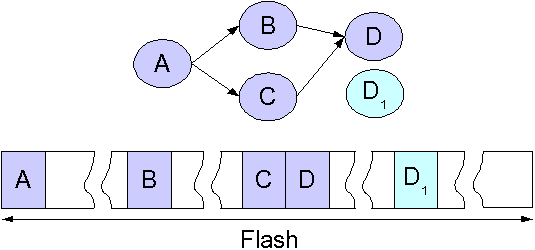
\includegraphics{pics/idxprobl.png}
\end{htmlonly}
%begin{latexonly}
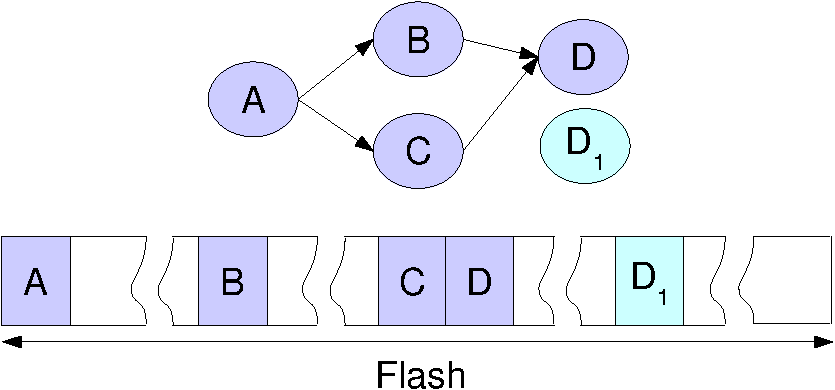
\includegraphics[width=100mm,height=50mm]{pics/idxprobl.pdf}
%end{latexonly}
\end{center}
\caption{JFFS3 indexing problem example.}
\label{ref_FigureIndexProblem}
\end{figure}

Suppose the index is kept and maintained on flash and it consists of 4
parts $A$, $B$, $C$, and $D$ which refer each other: $A$ refers $B$ and $C$,
$B$ refers $D$, and $C$ refers $D$. This means, that $A$ contains the physical
flash address of $B$ and $C$ and so on.

Suppose $D$ should be updated. Since it is updated \mbox{out-of-place}, the
newer version $D_1$ is written to some other place. But there are $B$ and $C$
which still refer $D$, not $D_1$, and they ought to be updated as well. And
when they are updated \mbox{out-of-place}, $A$ will still refer the old $B$ and
$C$, and so on. Thus, it is not that trivial to store and maintain indexing
information on the flash media.

%
% WANDERING TREES
%
\subsection{Wandering trees} \label{ref_SectionWandTrees}

To address the above problem it is possible to use \emph{wandering trees}.
Figure \ref{ref_FigureWandtree} demonstrates how do wandering trees work.

%
% Figure with the wandering tree example
%
\begin{figure}[h]
\begin{center}
\begin{htmlonly}
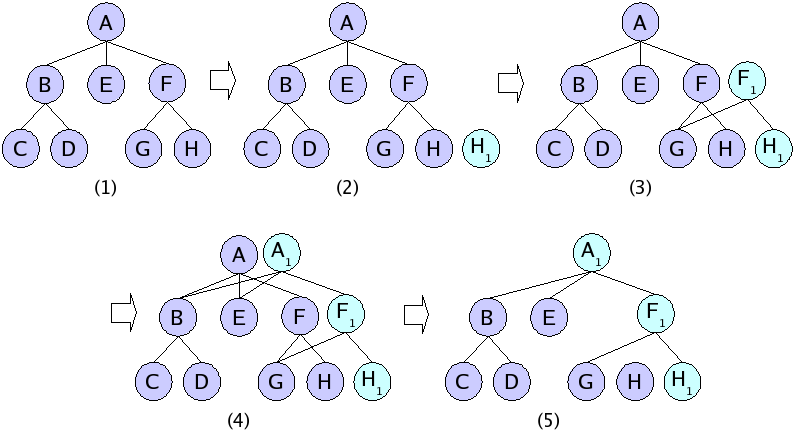
\includegraphics{pics/wandtree.png}
\end{htmlonly}
%begin{latexonly}
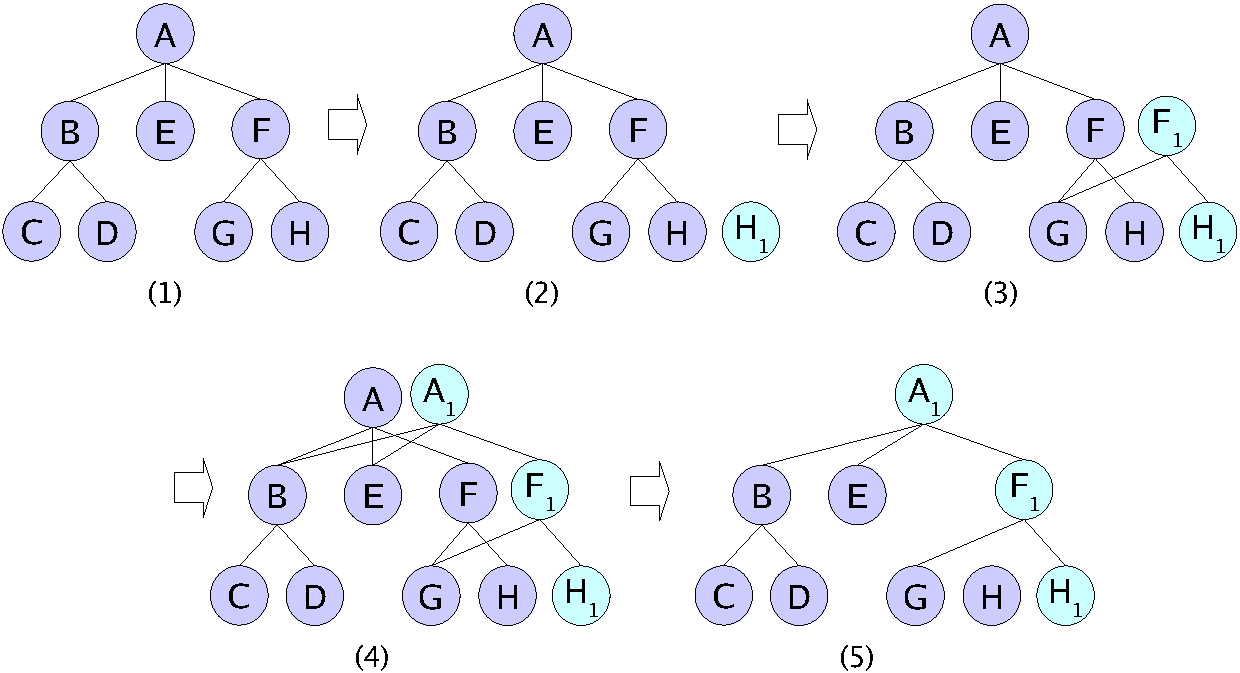
\includegraphics[width=159mm,height=80mm]{pics/wandtree.pdf}
%end{latexonly}
\end{center}
\caption{Wandering tree example.}
\label{ref_FigureWandtree}
\end{figure}

\begin{enumerate}

\item Suppose that the index is a tree and it is stored and maintained
on the flash media. The tree consists of nodes
$A$, $B$, $C$, $D$, $E$, $F$, $G$, and $H$.
Suppose node $H$ should be updated.

\item At first, the updated version $H_1$ is written. Obviously, $F$ still
refers $H$.

\item Now the corresponding link in node $F$ is changed and node $F_1$ is
written to flash. $F_1$ refers $H_1$. But as $F_1$ is also written
\mbox{out-of-place}, $A$ still refers the old node $F$.

\item Finally, the new root node $A_1$ is written ant it refers $F_1$.

\item Nodes $A$, $F$, $H$ are now treated as garbage and the updated tree is
composed by nodes $A_1$, $B$, $C$, $D$, $E$, $F_1$, $G$, and $H_1$.

\end{enumerate}

So, wandering trees is the base idea of how the indexing information is going
to be maintained on the flash media in JFFS3. And it stands to reason that any
tree may be called "wandering tree" if any update in the tree requires updating
parent nodes up to the root. For example, it makes sense to talk about
wandering \mbox{Red-Black} trees or wandering \mbox{$B^+$-trees} and so forth.

%
% B+ TREES
%
\subsection{B-trees} \label{ref_SectionBTrees}

JFFS3 uses \mbox{$B^+$-trees} and this subsection makes a short introduction to
\mbox{$B^+$-trees}. There is a plenty of books where one may find more
information.

The inexact definition of \mbox{$B$-tree} may be formulated as a balanced
search tree where each node may have many children. The \emph{branching factor}
or the \emph{fanout} defines the maximal number of node's children. While
\mbox{$B$-trees} may contain both useful data and \emph{keys} and \emph{links}
in \mbox{non-leaf} nodes, \mbox{$B^+$-trees} are \mbox{$B$-trees} which store
data only in leaf nodes, while \mbox{non-leaf} nodes contain only keys and
links.

%
% The figure with B+-tree example
%
\begin{figure}[h]
\begin{center}
\begin{htmlonly}
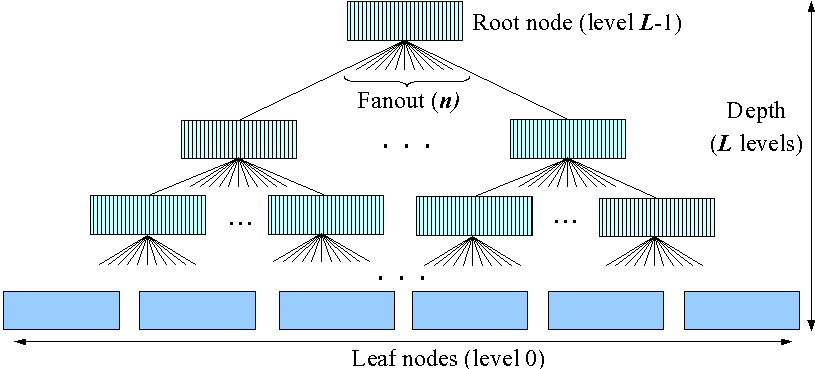
\includegraphics{pics/btree-01.png}
\end{htmlonly}
%begin{latexonly}
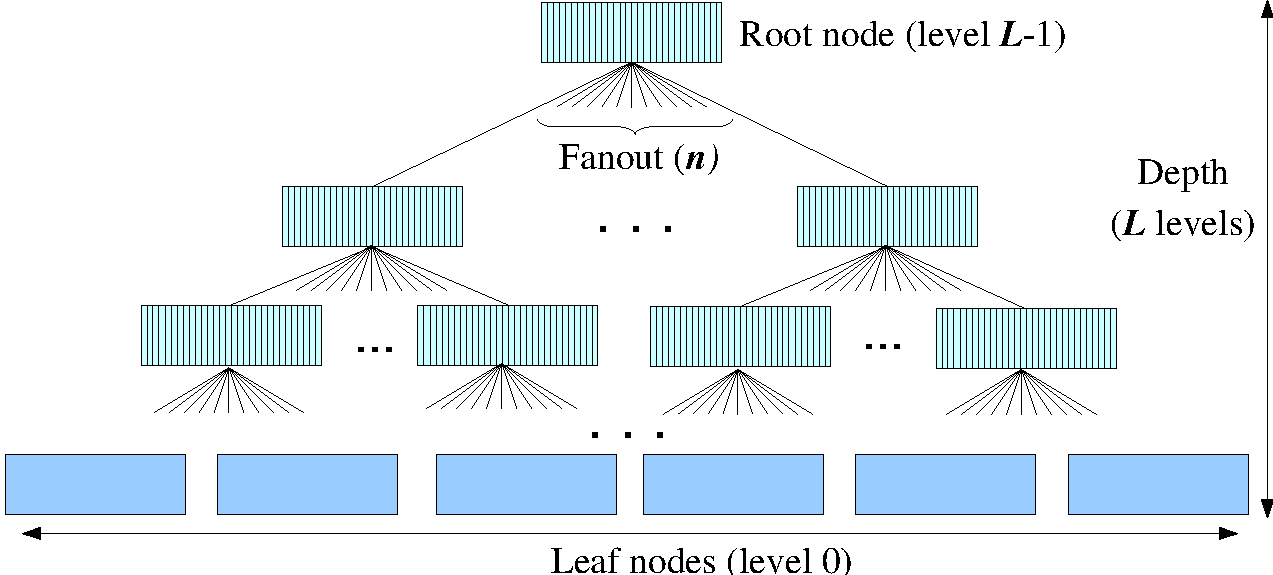
\includegraphics[width=159mm,height=65mm]{pics/btree-01.pdf}
%end{latexonly}
\end{center}
\caption{$B^+$-tree example.}
\label{ref_FigureBTree_01}
\end{figure}

Figure \ref{ref_FigureBTree_01} demonstrates a \mbox{$B^+$-tree} with branching
factor $n$ and the number of level $L$. Note, that in JFFS3 levels are numbered
starting from \emph{leaf} nodes (level 0) and ending at the \emph{root} node
(level $L-1$).

Leaf nodes in the \mbox{$B^+$-tree} contain data which are indexed by
keys. \mbox{Non-leaf} nodes do not contain data, but contain only the indexing
information, namely, \emph{keys} and \emph{links}.

%
% Figure with B+-tree non-leaf node
%
\begin{figure}[h]
\begin{center}
\begin{htmlonly}
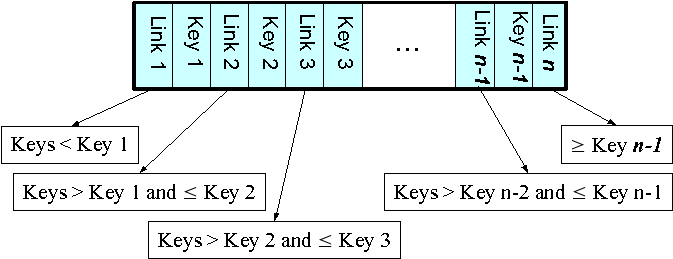
\includegraphics{pics/node-01.png}
\end{htmlonly}
%begin{latexonly}
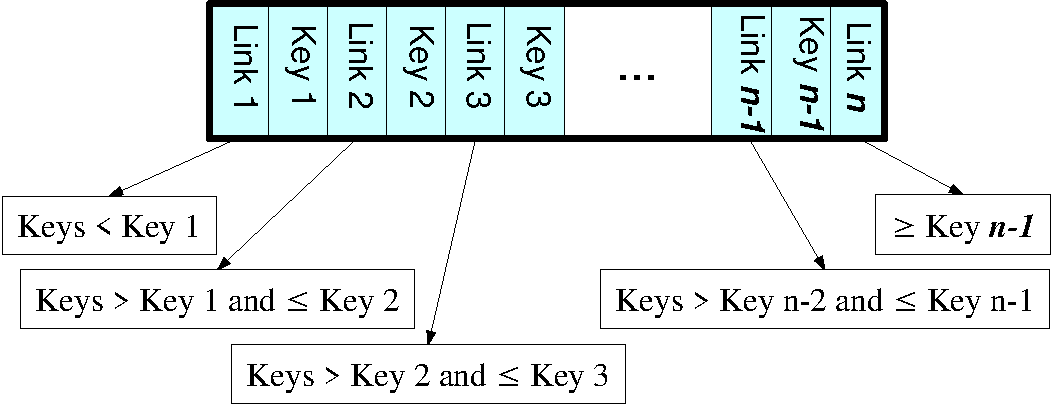
\includegraphics[width=160mm,height=60mm]{pics/node-01.pdf}
%end{latexonly}
\end{center}
\caption{The structure of a non-leaf node in $B^+$-tree.}
\label{ref_FigureNode_01}
\end{figure}

Figure \ref{ref_FigureNode_01} depicts the structure of a \mbox{non-leaf}
node. There are $n$ links and $n-1$ keys in the node. Links may point to either
leaf nodes or other \mbox{non-leaf} nodes. In the former case, the leaf node
will contain data which corresponds to the key which follows the link. In the
latter case, the pointed \mbox{non-leaf} node (and the whole subtree with the
root in this \mbox{non-leaf} node) will contain more keys in range
$(Key~1, Key~2]$.

Keys are sorted in the ascending order in \mbox{non-leaf} nodes, so it is not
that difficult to lookup data corresponding to any key. Furthermore, the tree
is balanced, so the the number of lookup steps does not depend on the key.

When objects are inserted or removed from the tree, \mbox{re-balancing} may be
needed. The tree is \mbox{re-balanced} by means of splitting nodes or merging
them and there is a simple enough algorithm exists. Please, refer to Donald
Knuth's books for more information about \mbox{re-balancing}
\mbox{$B^+$-trees}.

\mbox{$B^+$-trees} are widely used when working with block devices (e.g., hard
drives). Indeed, these devices have a fixed input/output unit size (usually
referred to as a \emph{sector}) and it is natural to use \mbox{$B^+$-trees}
with node size multiple to the size of the sector in order to store information
on such devices.

%
% INDEXING IN JFFS3
%
\subsection{Indexing in JFFS3} \label{ref_SectionIndexing}

The way how JFFS3 stores and indexes the file system is similar to the approach
used by the \emph{Reiser4} file system (see [\ref{ref_Reiser4}]). All the file
system objects (inodes, files, directory entries, extended attributes, etc) are
kept in one large \mbox{$B^+$-tree}. Effectively, the whole JFFS3 file system
may be regarded as one large \mbox{$B^+$-tree}.  This tree is further referred
to just as "\emph{the tree}".

Every object which is stored in the tree has a \emph{key}, and the object is
found in the tree by this key. To make it clearer what are object keys, the
following is an example of how they may look like:

\begin{itemize}

\item file data key: \{\texttt{inode number}, \texttt{offset}\};

\item directory entry key: \{\texttt{parent directory inode number},
\texttt{direntry name hash}\};

\item extended attribute key: \{\texttt{target inode number}, \texttt{xattr
name hash}\} and the like.

\end{itemize}

The following are terms which are used in JFFS3 to refer nodes of different
levels in the tree:

\begin{itemize}

\item nodes of level 0 are \emph{leaf nodes};

\item nodes of level 1 are \emph{twig nodes};

\item nodes which are not the root, not leaf, and not twig are \emph{branch
nodes};

\item \mbox{no-leaf} nodes (i.e., the root, branch and twig) are
\emph{indexing nodes}.

\end{itemize}

Note, the same terminology (except indexing nodes) is used in the Reiser4 file
system~[\ref{ref_Reiser4}].

\mbox{Non-leaf} nodes are called "indexing nodes" because they contain only
indexing information, nothing else. No file system data is kept in the indexing
nodes. Indexing nodes have fixed size which is equivalent to the flash
\emph{sector} size.

It is important to note that somewhat unusual terminology is used in this
document. The smallest input/output unit of the flash chip is called a
\emph{sector}. Since JFFS3 mainly orients to NAND flashes, the sector is mostly
the NAND page and is either 512 bytes or 2 Kilobytes. For other flash types the
sector may be different. If flash's minimal input/output unit is very small
(say, one bit as in case of NOR flash), there should be a layer which emulates
larger sectors (say, 512 bytes).

In opposite to indexing nodes, leaf nodes have flexible size, just like nodes
in JFFS2. So, roughly speaking, JFFS3 file system may be considered as JFFS2
file system (leaf nodes) plus indexing information (indexing nodes) (see figure
\ref{ref_FigureBTree_02}). 

%
% Figure the JFFS3 tree example
%
\begin{figure}[h]
\begin{center}
\begin{htmlonly}
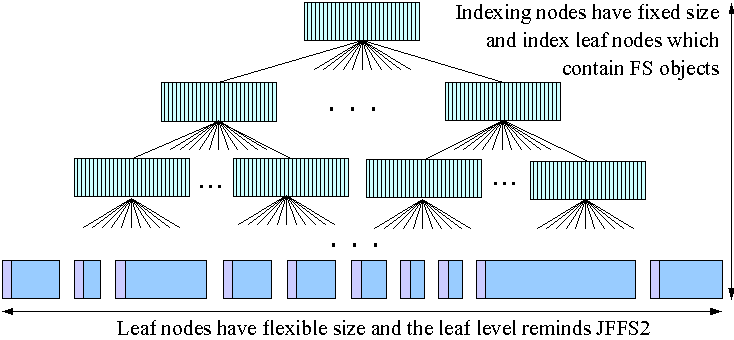
\includegraphics{pics/btree-02.png}
\end{htmlonly}
%begin{latexonly}
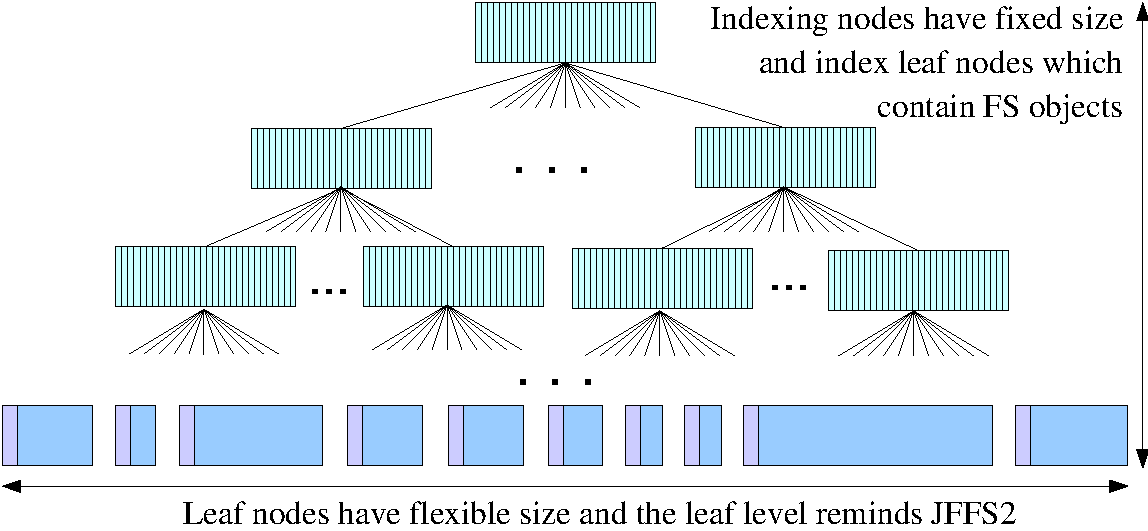
\includegraphics[width=159mm,height=70mm]{pics/btree-02.pdf}
%end{latexonly}
\end{center}
\caption{The JFFS3 tree.}
\label{ref_FigureBTree_02}
\end{figure}

Similarly to JFFS2, leaf nodes consist of \emph{header} and \emph{data}. The
header describes the node data and contains information like the key of the
node, the length, and the like. Node data contains some file system data, for
example a directory entry, file's contents, etc. 

Leaf and indexing nodes are physically separated, which means that there are
eraseblocks with only indexing nodes and with only leaf nodes. But of course,
this does not mean that the whole flash partition is divided on two parts, this
only means that the indexing and leaf nodes are not in one eraseblock. Figure
\ref{ref_FigureFlash_01} illustrates this.

%
% Figure with demonstration leaf and indexing nodes separation.
%
\begin{figure}[h]
\begin{center}
\begin{htmlonly}
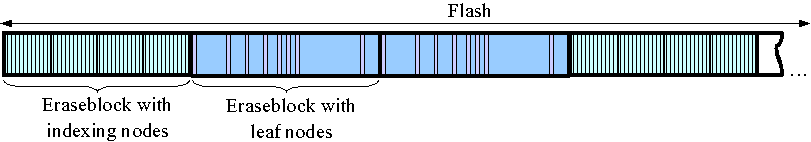
\includegraphics{pics/flash-01.png}
\end{htmlonly}
%begin{latexonly}
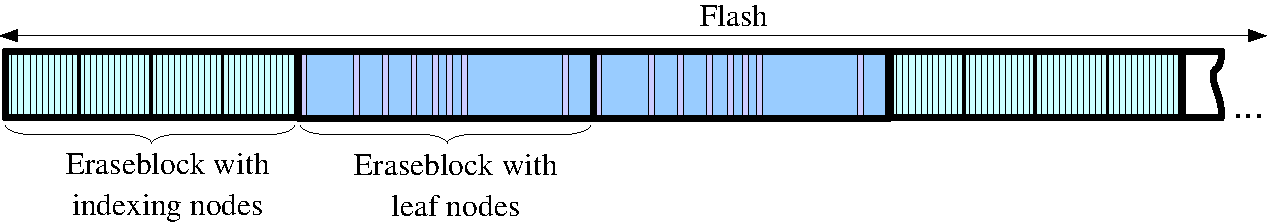
\includegraphics[width=159mm,height=30mm]{pics/flash-01.pdf}
%end{latexonly}
\end{center}
\caption{Illustration of leaf and indexing nodes separation.}
\label{ref_FigureFlash_01}
\end{figure}

Eraseblocks which contain only indexing nodes are called \emph{indexing
eraseblocks} and those with leaf nodes are called \emph{leaf eraseblocks}.

The depth of the tree depends on how many objects are kept on the file system.
The more files, directories, etc are present on the file system, the deeper is
the tree. Fortunately, the number of tree levels grows very slowly with the
growing number of file system objects and the tree lookup scales as
$O(log_n{S})$ (logarithmically).

The following are advantages of the JFFS3 indexing approach.

\begin{itemize}

\item Many different key assignment schemes may be used and this gives a
flexibility in how objects are sorted in the tree. Thus, one may optimize JFFS3
for specific workloads by means of changing the format of the keys.

\item Leaf nodes may be compressed, so JFFS3 admits of the \mbox{on-flight}
compression.

\item In case of corruptions of the indexing information it is possible to
\mbox{re-create} it by means of scanning leaf nodes' headers.

\item There is a clear separation between data and indexing information. This
implies that the indexing information and data may be cached separately,
without overlapping in the same cache lines. This leads to better cache usage
as described in the Reiser4 paper~[\ref{ref_Reiser4}].

\end{itemize}

%
% THE JOURNAL
%
\subsection{The Journal} \label{ref_SectionJournalIntro}

The JFFS3 tree is both \mbox{$B^+$-tree} and wandering tree. Any file system
change implies that a new node is written to the flash media, which in turn,
assumes that a number of indexing nodes must be updated. Namely, the whole path
of indexing nodes up to the root node should be updated (see section
\ref{ref_SectionWandTrees}).

Evidently, it is very expensive to update several indexing nodes on each file
system change and \emph{the journal} provides a mechanism to avoid this.

The journal consists of a set of eraseblocks (the \emph{journal eraseblocks})
which do not have a fixed location on flash and are not contiguous on flash.
Any flash eraseblock may be used as an journal eraseblock.

%
% The figure with journal illustration
%
\begin{figure}[h]
\begin{center}
\begin{htmlonly}
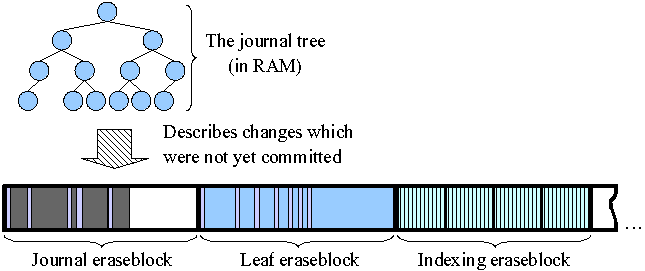
\includegraphics{pics/journal-01.png}
\end{htmlonly}
%begin{latexonly}
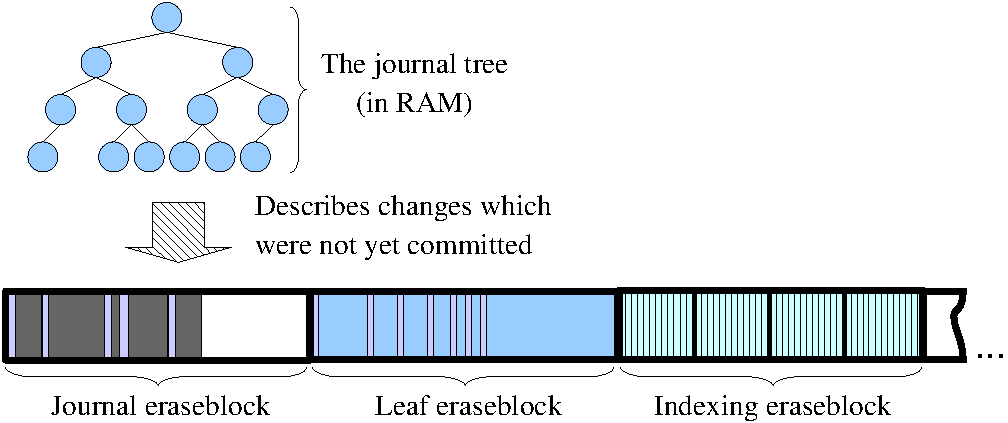
\includegraphics[width=159mm,height=65mm]{pics/journal-01.pdf}
%end{latexonly}
\end{center}
\caption{The JFFS3 journal.}
\label{ref_FigureJournal_01}
\end{figure}

When something is changed in the JFFS3 file system, the corresponding leaf node
is written to the journal, but the corresponding indexing nodes are not
updated. Instead, JFFS3 keeps track of file system changes in RAM in a data
structure called \emph{the journal tree} (see figure
\ref{ref_FigureJournal_01}).

When something is read from the file system, JFFS3 first glimpses at the
\mbox{in-RAM} journal tree to figure out if the needed data is in the journal.
If the data are  there, the journal is read, otherwise JFFS3 performs the usual
tree lookup (see figure \ref{ref_FigureJournal_02}).

%
% Figure with write request
%
\begin{figure}[h]
\begin{center}
\begin{htmlonly}
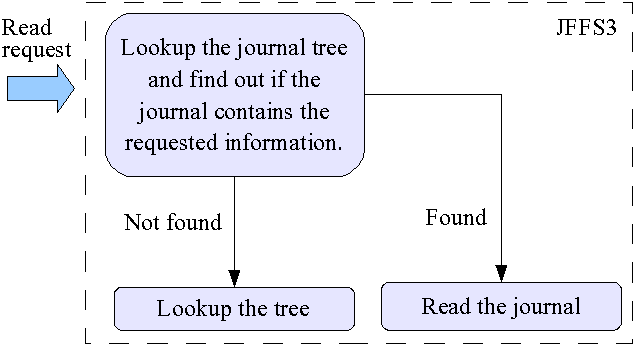
\includegraphics{pics/journal-02.png}
\end{htmlonly}
%begin{latexonly}
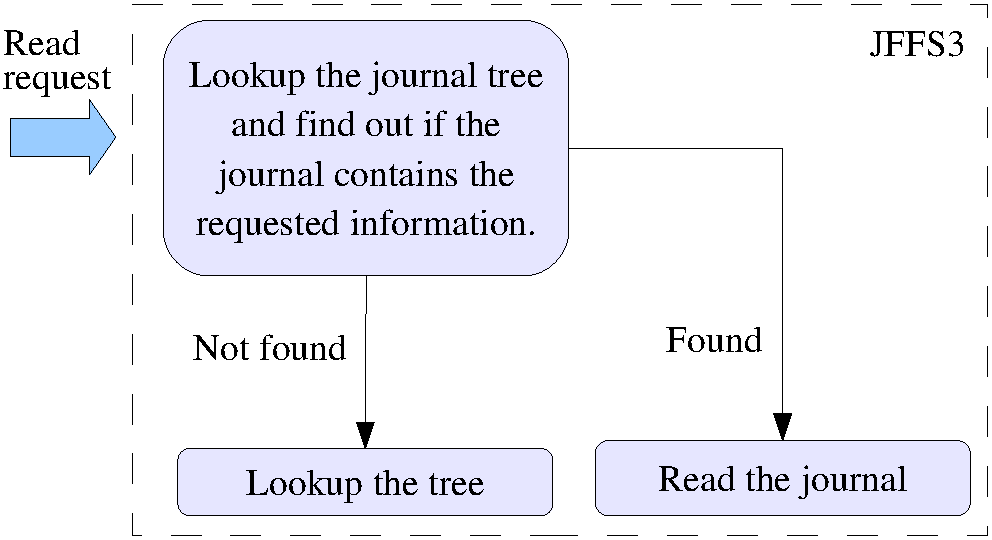
\includegraphics[width=130mm,height=60mm]{pics/journal-02.pdf}
%end{latexonly}
\end{center}
\caption{The read request processing in JFFS3.}
\label{ref_FigureJournal_02}
\end{figure}

The journal is \emph{committed} when it is full or in some other appropriate
for JFFS3 time. This means, that the indexing nodes corresponding to the
journal changes are updated and written to the flash.  The committed
journal eraseblocks are then treated as leaf eraseblocks and new journal
eraseblocks are picked by JFFS3 using the common JFFS3
\mbox{wear-levelling} algorithm.

The journal makes it possible to postpone indexing information updates to later
and potentially more appropriate time. It also allows to merge many indexing
node updates and lessen the amount of flash write operations.

When JFFS3 file system is being mounted, the journal should be read, "replayed"
and the journal tree should be built. So, the larger is the journal, the longer
it may take to mount JFFS3. From the other hand, the larger is the journal, the
more writes may be deferred and the better performance may be achieved. By the
other words, there is a \mbox{trade-off} between the mount time and the
performance and one may vary these characteristics by means of changing the
size of the journal.

\subsection{The superblock}

The JFFS3 \emph{superblock} is a data structure that describes the file system
as a whole and contains important information like the offset of the root node,
the journal eraseblocks, etc. When the file system is being mounted, it first
finds and reads the JFFS3 superblock.

In case of traditional file systems the superblock usually resides at a fixed
position on the disk and may be found very quickly. Conversely, due to the
"\mbox{out-of-place} write" flash property it is impossible to assign a fixed
position for the JFFS3 superblock. Things are getting even more complex because
of the need to provide good \mbox{wear-levelling}~-- it is incorrect to just
reserve several erasable blocks for the superblock unless it is guaranteed that
these eraseblocks will not be worn out earlier then the other eraseblocks.

We have the following two requirements that ought to be met in JFFS3:

\begin{itemize}

\item JFFS3 must be able to quickly find the superblock;

\item the superblock management techniques must not spoil the overall flash
wear levelling.

\end{itemize}

In the classical file systems the superblock usually contains a lot of static
data which is rarely updated and the superblock may have any size. In JFFS3,
the superblock must be updated quite often (e.g., each time the journal is
committed). This means that to lessen the amount of I/O, the JFFS3 superblock
should be as small as it is possible, namely, one sector. And there is no
reason to keep any static data in the superblock (e.g., the size of the file
system, its version, etc). For static data, JFFS3 reserves the first eraseblock
of the JFFS3 partition.

Thus, the following terms are used in this document:

\begin{itemize}

\item \emph{static superblock}~-- contains only static data which are never
changed by JFFS3; the static superblock resides at the \emph{static
eraseblock}; the static eraseblock is the first \mbox{non-bad} eraseblock of
the JFFS3 partition; it is supposed that the contents of the static eraseblock
may only be changed by external \mbox{user-level} tools;

\item \emph{superblock}~-- contains only dynamic data, is changed quite
often and requires special methods to deal with.

\end{itemize}

JFFS3 has a rather complicated superblock management scheme which makes it
possible to quickly find the superblock without full flash scanning when the
file system is being mounted. This scheme provides good flash
\mbox{wear-levelling}. The superblock lookup should take few milliseconds and
scale as $O(log_2(S))$. For more detailed information about the superblock
management scheme see section \ref{ref_SectionSBAlg}.

%%%%%%%%%%%%%%%%%%%%%%%%%%%%%%%%%%%%%%%%%%%%%%%%%%%%%%%%%%%%%%%%%%%%%%%%%%%%%%%%
%
% THE SUPERBLOCK
%
%%%%%%%%%%%%%%%%%%%%%%%%%%%%%%%%%%%%%%%%%%%%%%%%%%%%%%%%%%%%%%%%%%%%%%%%%%%%%%%%
\section{The superblock}

%
% THE SUPERBLOCK MANAGEMENT ALGORITHM
%
\subsection{The superblock management algorithm} \label{ref_SectionSBAlg}

To implement the superblock management scheme, JFFS3 reserves the second and
the third good eraseblocks at the beginning of the flash partition (just next
to the static eraseblock). These two eraseblocks are called \emph{anchor
eraseblocks}, or the \emph{anchor area}.

Anchor eraseblocks contain references to \emph{chain eraseblocks}. Chain
eraseblocks may either refer other chain eraseblocks or the \emph{super
eraseblock} (see figure \ref{ref_FigureSB_01}). The number of chain eraseblocks
varies depending on the size of the JFFS3 partition. If there are $k$ chain
erase blocks, the anchor area will refer chain eraseblock 1, which will refer
chain eraseblock 2, which will refer chain eraseblock 3 and so forth. The chain
eraseblock $k$ will refer the super eraseblock.

%
% Figure with superblock management superblocks
%
\begin{figure}[h]
\begin{center}
\begin{htmlonly}
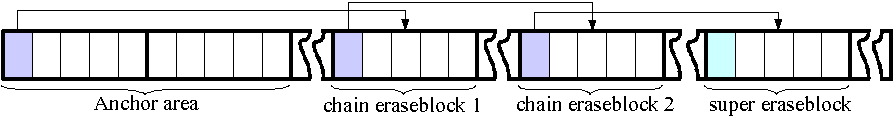
\includegraphics{pics/sb-01.png}
\end{htmlonly}
%begin{latexonly}
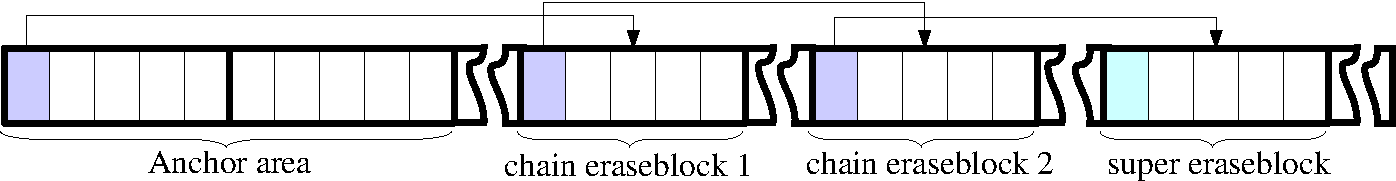
\includegraphics[width=159mm,height=21mm]{pics/sb-01.pdf}
%end{latexonly}
\end{center}
\caption{Types of eraseblocks involved to the superblock management scheme.}
\label{ref_FigureSB_01}
\end{figure}

The super eraseblock contains the superblock which takes \emph{one sector}. The
chain eraseblocks contain references to the next chain eraseblock or to the
super eraseblock.

The JFFS3 superblock management mechanisms work as follows. Suppose there are
$k$ chain eraseblocks in the current superblock management scheme. The superblock
updates are written to consecutive sectors of the super eraseblock. When
the super eraseblock has no more empty sectors, new super eraseblock is picked,
the superblock update is written to the new super eraseblock, and new reference
is written to the chain eraseblock~$k$.

Similarly, when there is no space in the chain eraseblock~$k$, new chain
eraseblock~$k$ is picked and the corresponding reference is written to chain
eraseblock~$k-1$, and so on. When there are no free sectors in the chain
eraseblock~1, new chain eraseblock~1 is picked and the corresponding
reference is written to the anchor area.

Figure \ref{ref_FigureSB_02} presents the example of the superblock management
scheme ($k = 2$).

%
% Superblock management example
%
\begin{figure}[!t]
\begin{center}
\begin{htmlonly}
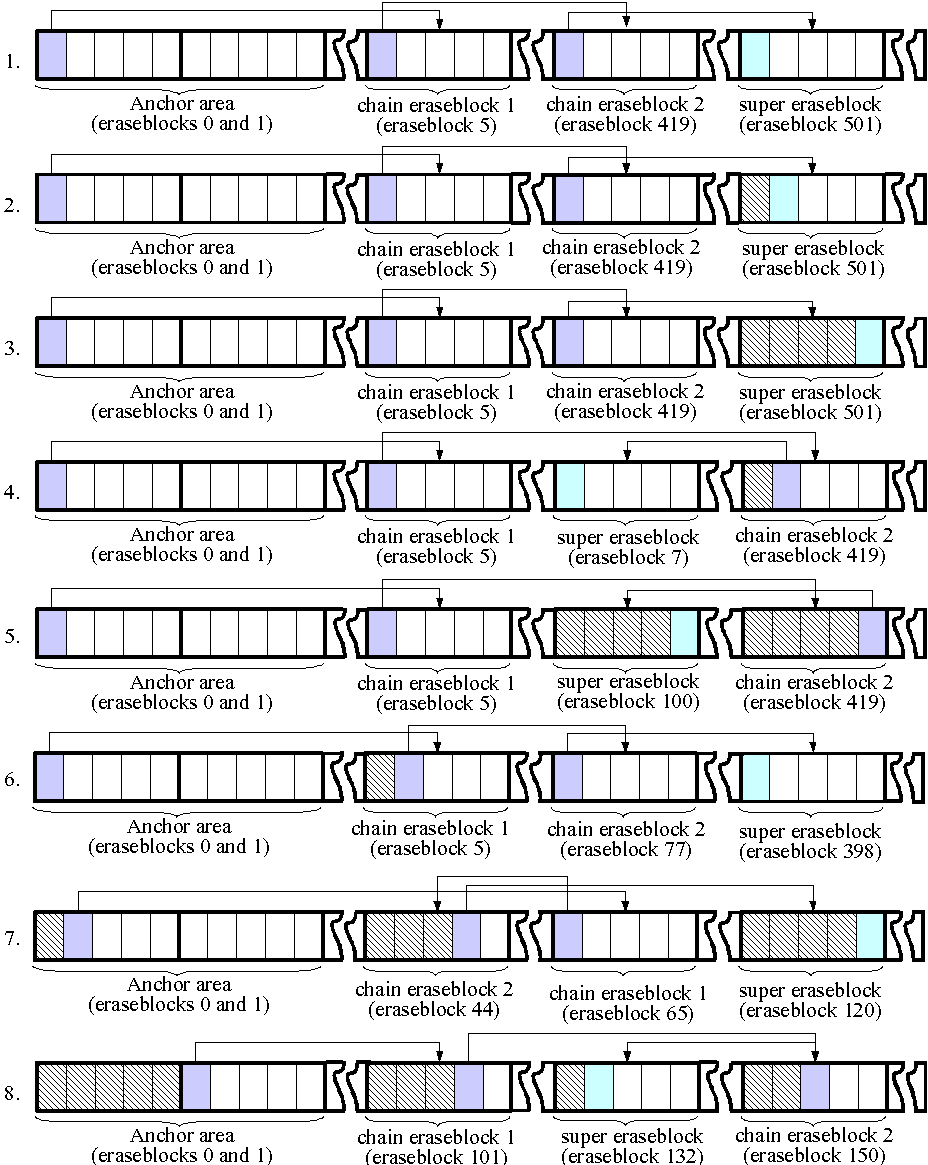
\includegraphics{pics/sb-02.png}
\end{htmlonly}
%begin{latexonly}
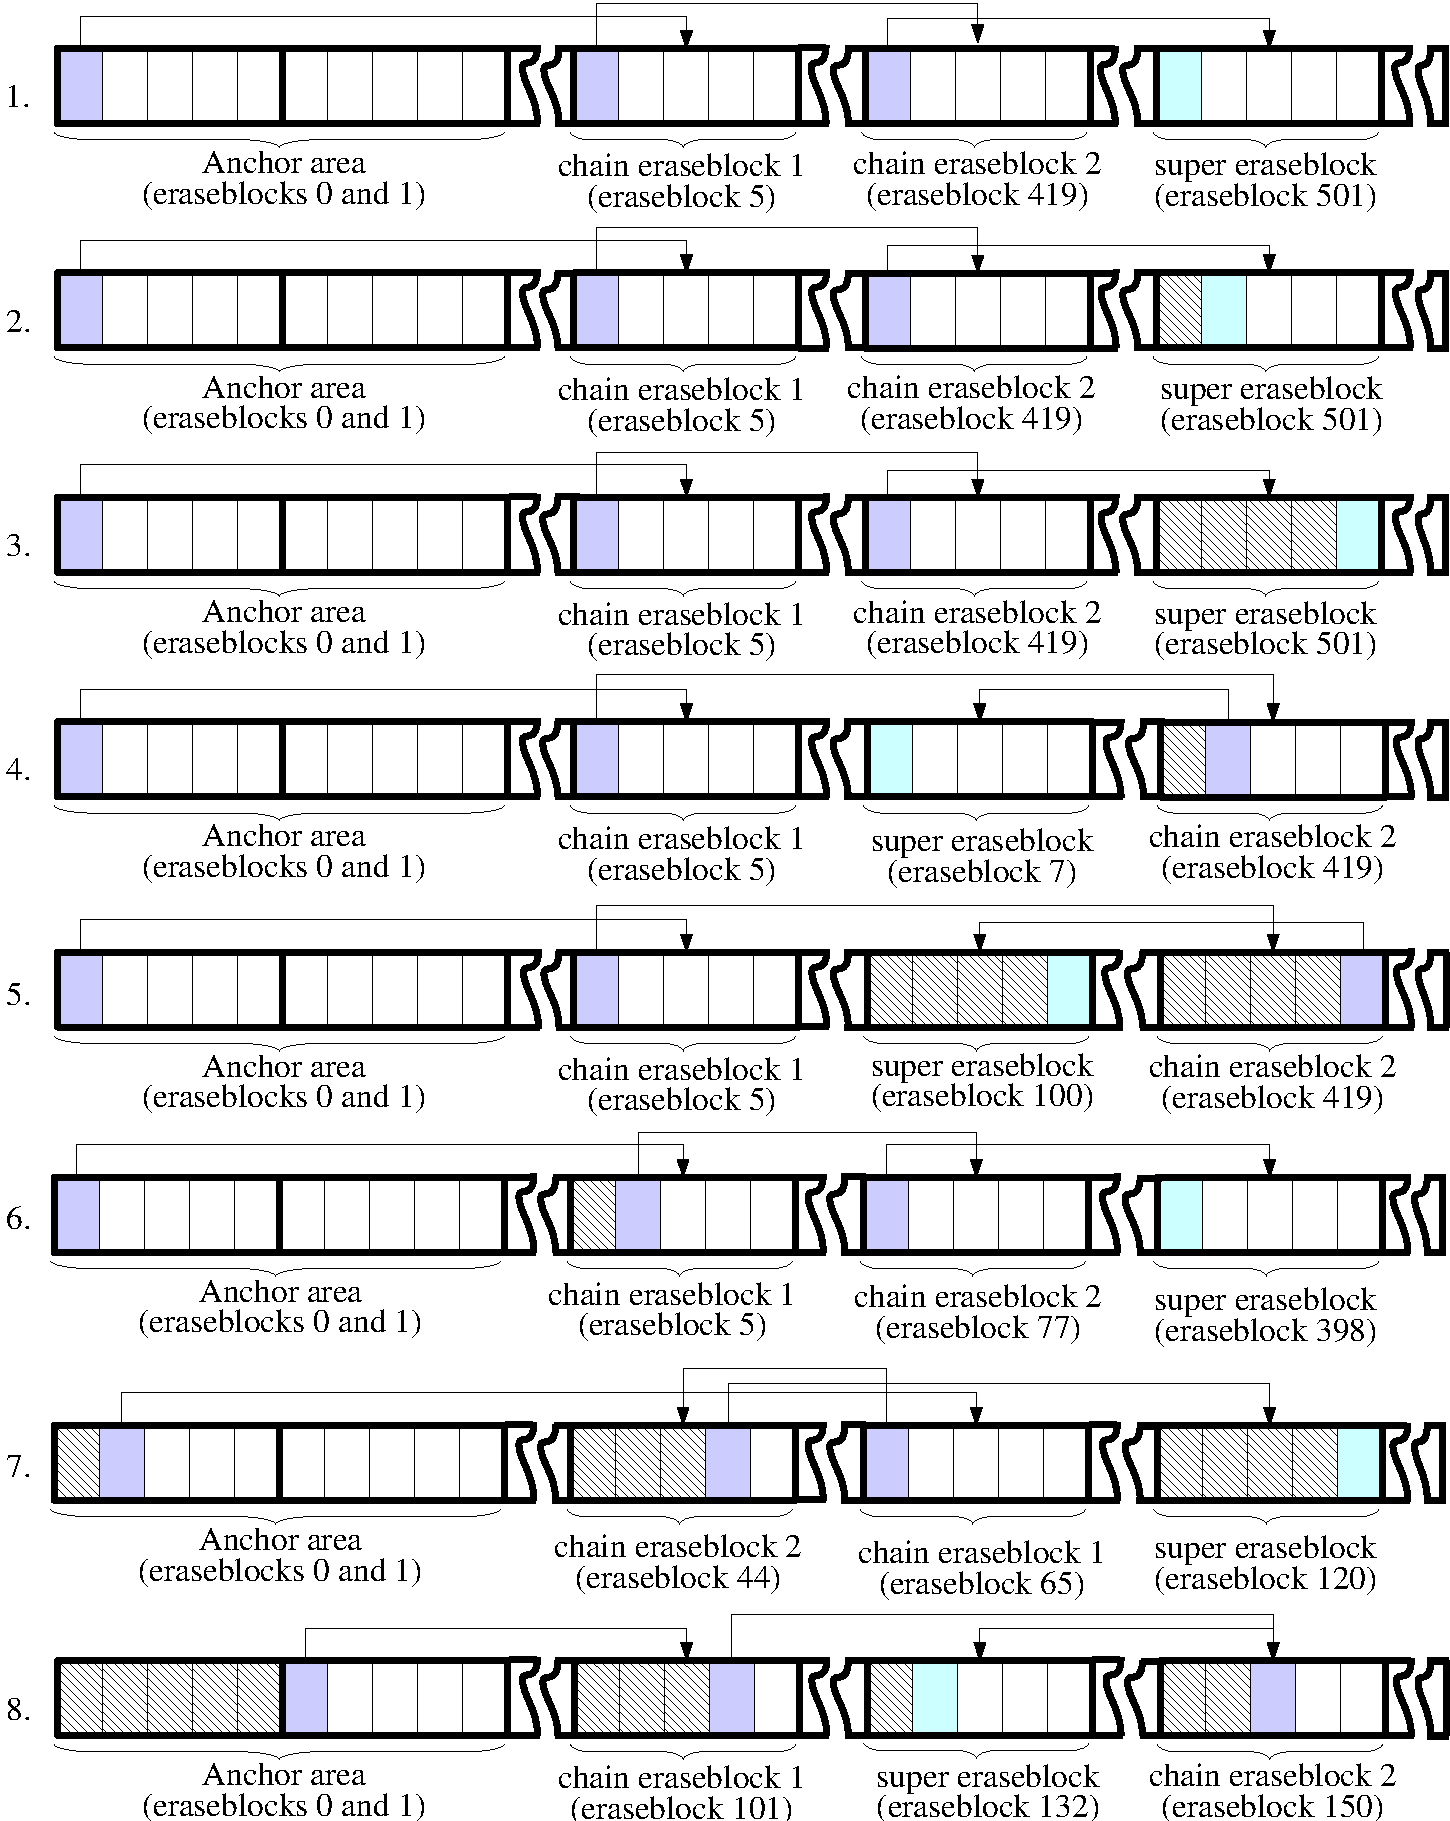
\includegraphics[width=159mm,height=200mm]{pics/sb-02.pdf}
%end{latexonly}
\end{center}
\caption{The superblock management example.}
\label{ref_FigureSB_02}
\end{figure}

\begin{enumerate}

\item Initially, there are 2 chain eraseblocks (numbers 5 and 419) and the super
eraseblock (number~501). There is a reference in the first sector of the anchor
area which refers the chain eraseblock~1. The first sector of the chain
eraseblock~1 refers the chain eraseblock~2, and the first sector of the chain
eraseblock~2 refers the super eraseblock. The first sector of the super
eraseblock contains the superblock.

\item After the superblock has been updated, the second sector of the super
eraseblock contains the valid copy of the superblock and the first sector
contains garbage.

\item The superblock has been updated many times and the valid superblock is at
the last sector of the super eraseblock while the other sectors of the super
eraseblock contain garbage.

\item As there were no free sectors at the super eraseblock, new super
eraseblock was chosen (eraseblock number~7) and the superblock update was
written to the first sector of the new super eraseblock. As the super
eraseblock changed its position, the corresponding reference at the chain
eraseblock~2 was updated. It was updated \mbox{out-of-place} and now the first
sector of the chain eraseblock~2 is dirty while the second sector contains the
valid reference to the new super eraseblock.

\item The superblock has been updated many times and the super eraseblock
changed its position many times and it is currently at the eraseblock number
100. The reference to the super eraseblock was also updated many times and at
the moment the last sector of the chain eraseblock~2 contains the valid
reference while the other sectors are obsolete. Similarly, the last sector of
the super eraseblock contains valid superblock while the other sectors are
obsolete.

\item When the next superblock update came, there were no free sectors at the
super eraseblock and new super eraseblock was picked (eraseblock number~398)
and the valid copy of the superblock is currently at the first sector of the
eraseblock number~398, Also, there were no free sectors at the chain
eraseblock~2 and new chain eraseblock~2 was picked (eraseblock number~77), so
the first sector of the eraseblock~77 contains the valid reference to the super
eraseblock. Since the chain eraseblock~2 changed its position, the
corresponding reference at the chain eraseblock~1 was updated and at the moment
the second sector of the chain eraseblock~1 contains the valid reference to the
chain eraseblock~2 while the first sector is dirty.

\item And analogously, after many superblock updates, the chain eraseblock~1
was updated many times and when it became full it changed its position.  Sure,
the chain eraseblock~2 and the super eraseblock changed their positions many
times as well. So, at the moment, the chain eraseblock~1 is at the eraseblock
number~65, the chain eraseblock~2 is at the eraseblock~44 and the super
eraseblock is at the eraseblock~120. When the chain eraseblock~1 changed its
position, the corresponding reference at the anchor area was updated and
currently the second sector of the anchor eraseblock~1 contains the valid
reference to the chain eraseblock~1 while the firs sector is dirty.

\item And even more superblock updates happened. The anchor area was updated
many times. When there were no free sectors at the anchor eraseblock~1, the
anchor eraseblock~2 was used. So, at the moment, the valid reference to the
chain eraseblock~1 is at the first sector of the anchor eraseblock~2. From now
on, the first anchor eraseblock may be erased and may be used again when the
second anchor eraseblock is full.

\end{enumerate}

The following are important notes about the JFFS3 superblock management.

\begin{itemize}

\item The superblock takes one sector so the super eraseblock may be updated at
most $N$ times ($N$ is the number of sectors in the eraseblock).

\item In case of NAND flash, the sector is the real minimal physical
input/output unit, so only $N$ updates are possible in anchor eraseblocks
and in chain eraseblocks. But if the real input/output unit is smaller then
the sector (i.e., if JFFS3 works on top of NOR flash) the advantage of this may
be used and more references may be packed into one anchor or chain eraseblock.

\item When JFFS3 picks new chain/super eraseblock, the common JFFS3
\mbox{wear-levelling} scheme is utilized.

\item Anchor area has 2 eraseblocks in order to ensure the tolerance to unclean
reboots~-- one anchor eraseblock may be safely erased while the other is being
used.

\item When a new reference is written to anchor/chain eraseblocks, the previous
reference becomes dirty and on mount JFFS3 should find the valid reference. To
facilitate this, each reference has its version number.  Each subsequent
reference has higher version then the previous. Hence, JFFS3 may use the
binary search algorithm to quickly find the valid reference.

\item As unclean reboot may happen anytime, no anchor/chain/super eraseblocks
are erased before the whole chain has been updated. This makes it possible to
recover from unclean reboots if they happen while the chain of the
\mbox{superblock-related} eraseblocks is being updated.

\end{itemize}

%
% THE LENGTH OF THE CHAIN
%
\subsection{The length of the chain}

The number of required eraseblocks in the superblock management scheme depends
on the size of the JFFS3 partition. The larger the partition, the more levels
are needed. This is determined by the need to ensure that the anchor area is
not worn out earlier then the rest of the JFFS3 partition.

Let's denote the number of required chain eraseblocks plus one (the super
eraseblock) $m$ and calculate $m$ assuming the worst case scenario: any
file system data update requires the superblock update. This would correspond
to synchronous JFFS3 operation mode with \mbox{zero-length} journal.

Obviously, what is wanted is to be sure that the anchor area is not worn out
earlier then the data area, i.e. the following inequality should be true:

\begin{equation}
\frac{T_A}{T_D} \geqslant 1,
\label{ref_EquationSBIneq}
\end{equation}

where $T_A$ is the period of time of the total anchor area wear and $T_D$ is
the period of time of the total data area wear. Note, the whole JFFS3 partition
excluding the static superblock and the anchor area is referred to as the
\emph{data area}.

If $R_A$ is the average rate of the anchor area updates (sectors per second),
$R_D$ s the average rate of the data area updates and $N$ is the number of
sectors per the eraseblock, then the anchor area will be written to with rate
$R_A/N$ eraseblocks per second and the data area will be written to with the
rate $R_D/N$ eraseblocks per second. So, JFFS3 will need to erase $R_A/N$
eraseblocks per second in the anchor area and $R_D/N$ eraseblocks per second in
the data area. Therefore, $T_A$ and $T_D$ may be expressed as

$$
T_A = \frac{2D \cdot N}{R_A},
$$
$$
T_D = \frac{(M-3) \cdot D \cdot N}{R_D},
$$

where $D$ is the maximum number of flash eraseblock erase cycles, and $M$ is
the number of non-bad eraseblock on the JFFS3 partition. We subtracted 3 from
$M$ to get the number of eraseblocks in the data area.

\begin{equation}
\frac{T_A}{T_D} = 2 \cdot \frac{R_D}{(M-3) \cdot R_A}.
\label{ref_Equation_TA_and_TD}
\end{equation}

If $m = 0$, i.e., there are no chain/super eraseblocks and the superblock is
stored in the anchor area, then taking into account
(\ref{ref_Equation_TA_and_TD}) and that in this case $R_A = R_D = R$, we have

$$
\frac{T_A}{T_D} = \frac{2}{(M-2)}.
$$

Suppose $m = 1$. i.e., there are no chain eraseblocks and only the super
eraseblock is used. In this case each file system data update will require (a)
the superblock update in the data area and (b) the anchor area update.
Therefore, the anchor area will be written $N$ times less frequently then when
$m = 0$ and the data area will be written $2$ times more frequently then when
$m = 0$. This means, that $R_A = R/N$ and $R_D = 2R$ and from
(\ref{ref_Equation_TA_and_TD}) we have

$$
\frac{T_A}{T_D} = 2 \cdot \frac{2N}{M-3}.
$$

When $m = 2$, i.e. the chain eraseblock 1 and the super eraseblock are used,
the anchor area will be written $N^2$ times less frequently, while the data
area will be written $2+1/N$ times more frequently then when $m = 0$ (one
superblock update on each file system update and one chain eraseblock 1 update
per $N$ superblock updates). Therefore, $R_A=R/N^2$ and $R_D = (2 + 1/N) \cdot
R$ and from (\ref{ref_Equation_TA_and_TD}) we have

$$
\frac{T_A}{T_D} = 2 \cdot \frac{2N^2+N}{M-3}.
$$

For $m = 3$, analogously,

$$
\frac{T_A}{T_D} = 2 \cdot \frac{2N^3 + N^2 + N}{M-3},
$$

and for $m = 0,1,2,\ldots$

$$
\frac{T_A}{T_D} = 2 \cdot \frac{2N^m + N^{m-1} + \ldots + N}{M-3}.
\label{ref_Equation_TA_div_TD}
$$

Consequently, from (\ref{ref_EquationSBIneq}) we have the following inequality:

$$
2 \cdot \frac{2N^m + N^{m-1} + \ldots + N}{M-3} \geqslant 1,
$$

or neglecting the minor components,

$$
\frac{4N^m}{M-3} \geqslant 1,
$$

or

\begin{equation}
m \geqslant log_N{\frac{M-3}{4}}.
\label{ref_EquationSBIneq1}
\end{equation}

Thus, form (\ref{ref_EquationSBIneq1}) it is obvious that the JFFS3 superblock
management scheme scales logarithmically.

Table \ref{ref_TableNANDLevels} shows the value of $m$ for different types of
existing NAND flashes.

\begin{table}[h]
\begin{center}
\begin{tabular}{llllll}
\textbf{Type} & \textbf{Size} & \textbf{Sect. size} & $\bf M$ & $\bf N$ &
\textbf{$\bf m$}\\
\hline
Toshiba TC58DVM92A1FT   & 64MB  & 16KB  & 4096  & 32 & 2\\
Toshiba TH58NVG1S3AFT05 & 512MB & 128KB & 4096  & 64 & 2\\
ST Micro NAND08G-B      & 1GB   & 128KB & 8192  & 64 & 2\\
Samsung K9K1G08X0B      & 2GB   & 128KB & 16384 & 64 & 2\\
\end{tabular}
\caption{The length of the JFFS3 superblock management chain for different
types of existing NAND flashes.}
\label{ref_TableNANDLevels}
\end{center}
\end{table}

Note, providing that $N=64$, $m=3$ is enough to guarantee acceptable anchor
area wear leveling for up to 128GB flash, $m=4$~-- for up to 8TB flash (the
inequality \ref{ref_EquationSBIneq1}).

%
% THE SUPERBLOCK SEARCH
%
\subsection{The superblock search}

To find the superblock during mount, JFFS3 finds the valid reference in the
anchor eraseblocks, then finds the valid reference in chain erase blocks
$1$,~$2$,~$\ldots$,~$m-1$, and finally finds the valid superblock in the super
eraseblock.  Since JFFS3 assigns versions to records in anchor/chain/super
eraseblocks and the versions are increased by one on every update, the binary
search algorithm may be used to quickly find the valid sector.

The valid reference in the anchor area may be found after $log_2(2N)+2$ steps
(one step involves one sector read operation), the reference in chain/super
eraseblocks~-- after $log_2(N)+2$ steps. Thus, to find the superblock, JFFS3
must read

$$
S = 2m + log_2(2N) + (m - 1) \cdot log_2(N)
$$

sectors.

Table \ref{ref_TableNANDTimes} contains the approximate superblock search time
for different existing NAND flashes
\footnote{the calculated superblock search time doesn't contain the ECC/CRC
checking overhead as well as any other CPU overhead.}.

\begin{table}[h]
\begin{center}
\begin{tabular}{lllllll}
\textbf{Type} & \textbf{Size} & $\bf N$ & $\bf m$ & \textbf{Sect. read} & $\bf
S$ & \textbf{SB find}\\
\hline
Toshiba TC58DVM92A1FT & 64MB & 32 & 2 & $\sim$50$\mu$s  & 22 & $\sim$1.1ms\\
ST Micro NAND08G-B    & 1GB  & 64 & 2 & $\sim$130$\mu$s & 25 & $\sim$3.3ms\\
Samsung K9K1G08X0B    & 2GB  & 64 & 2 & $\sim$70$\mu$s  & 25 & $\sim$1.6ms\\
\end{tabular}
\caption{The superblock search time for different existing NAND flashes.}
\label{ref_TableNANDTimes}
\end{center}
\end{table}

For larger flash chips which would utilize the superblock management scheme
with $m = 3$ (no such flashes exist at the moment), the superblock search time
would be about 4.3ms, providing the flash characteristics are the same as ST
Micro's (see table \ref{ref_TableNANDTimes}).

%%%%%%%%%%%%%%%%%%%%%%%%%%%%%%%%%%%%%%%%%%%%%%%%%%%%%%%%%%%%%%%%%%%%%%%%%%%%%%%%
%
% ISSUES/TO BE DONE
%
%%%%%%%%%%%%%%%%%%%%%%%%%%%%%%%%%%%%%%%%%%%%%%%%%%%%%%%%%%%%%%%%%%%%%%%%%%%%%%%%
\section{Issues/ideas/to be done}

This section contains a temporary list of issues which should be solved, ideas
which should be thought and analyzed deeper or things which were thought about
but are not yet described in this document.

The following is the list of things which should be thought about more.

\begin{enumerate}

\item Quota support. Will quota be supported? How will it look like -- lust
generic linux quota or something better?

\item Transactions:\\
\texttt{transaction\_open()/do\_many\_fs\_modifications()/transaction\_close()}
semantics? Reiser4 pretends to support this via special \texttt{sys\_reiser4()}
syscall. Would be nice.

\item Does it make sense to "compress" keys. For example, if there are many
consecutive keys with the same prefix, we may write this prefix only once. Will
there be some problems when these compressed keys are changed and cannot be
compressed any longer? Will this need some horrid tree and re-balancing?
The idea of "extents" is similar.

\item How can one select the compression mode on the per-inode basis? Xattrs
with some reserved name?

\item ACLs... Will they be implemented via xattrs or it will be something
tricker/better?

\item Orphaned files.

\item Holes.

\item Direct I/O.

\item When/how to update stat-data ?

\end{enumerate}

The following is the list of topics which should be highlighted in this document
as well.

\begin{enumerate}

\item Garbage collection.

\item Caching, write-behind cache.

\item An assumed flash model and the model of interactions between JFFS3 and
the flash I/O subsystem.

\item How the track of eraseblocks will be kept? Space accounting, good/bad,
erase count?

\item The wear-levelling algorithms.

\item The format of keys.

\item Branch nodes' links are sector numbers, twig nodes' links are absolute
flash offsets. So, the length of twig and branch keys are different and
branches have greater fanout.

\item Different optimizations may be achieved by means of changing the format
of keys. So, JFFS3 should be flexible in this respect and have a mechanism to
change/select the formats of keys.

\item The minimal amount of file's data in a node is \texttt{PAGE\_SIZE}. No
way to create smaller nodes as it it possible in JFFS2.

\end{enumerate}

The following is the list of ideas which were thought about but are not yet in
the document.

\begin{enumerate}

\item If the compression is disabled for an inode, then its nodes are
(\texttt{PAGE\_SIZE} + header size) in size, i.e., they do not fit into integer
number of flash sectors. For these nodes we may keep the header in the OOB
area. In this case we should not mix compressed nodes and uncompressed nodes in
one eraseblock.

\item For large files which are mostly read-only, we may fit more then one page
of data in one node. This will mace compression better. When the file is read,
all the uncompressed pages are propagated to the page cache, like in the zisofs
file system.

\item If there are few data in the superblock, we may keep this data in the
root node. In this case the root will have smaller fanout then branches.

\end{enumerate}

The "to do" list.

\begin{enumerate}

\item Re-calculate digits for SB search time and $m$.

\end{enumerate}

%%%%%%%%%%%%%%%%%%%%%%%%%%%%%%%%%%%%%%%%%%%%%%%%%%%%%%%%%%%%%%%%%%%%%%%%%%%%%%%%
%
% DEFINITIONS
%
%%%%%%%%%%%%%%%%%%%%%%%%%%%%%%%%%%%%%%%%%%%%%%%%%%%%%%%%%%%%%%%%%%%%%%%%%%%%%%%%
\section{Definitions}\label{ref_SectDefinitions}

\begin{enumerate}

\item \textbf{Access Control Lists, ACL}~-- a modern mechanism to control
accesses to files which provides much more flexibility that the standard Unix
mechanism of owner/group/others permissions, see [\ref{ref_ACL}] for more
details.

\item \textbf{Anchor eraseblock, anchor area}~-- the second and the third
\emph{good} eraseblocks of the JFFS3 partition which are reserved for the
superblock management. See section \ref{ref_SectionSBAlg} for more details.

\item \textbf{$B$-tree}~-- a balanced search tree where each node has many
children. See section \ref{ref_SectionBTrees}.

\item \textbf{$B^+$-tree}~-- a \mbox{$B$-tree} where no data is stored in
\mbox{non-leaf} nodes but instead, is stored only in leaf nodes.

\item \textbf{Branch node}~-- any node that is not leaf, not twig and not root.

\item \textbf{Branching factor}~-- the branching factor of the $B$-tree is the
number of children of a node.

\item \textbf{Chain eraseblock}~-- an eraseblock containing references to other
chain eraseblocks or to the super eraseblock. Chain eraseblocks facilitate
quick SB searching and are the part of the JFFS3 superblock management scheme
(see section \ref{ref_SectionSBAlg}). The main reason why chain eraseblocks are
needed is the need to provide good flash \mbox{wear-levelling}.

\item \textbf{Directory entry, direntry}~-- basically an association between
the name and the inode number. As any other object direntries are stored at the
leaf level of the tree in direntry nodes.

\item \textbf{Erasable block, eraseblock}~-- the minimal erasable unit of the
flash chip from the JFFS3's viewpoint.

\item \textbf{Extended attributes, xattr}~-- an association between names and
data for files and directories. See attr(5) Linux manual pages for more
information.

\item \textbf{Data area}~-- the whole JFFS3 partition excluding the static
superblock and anchor eraseblocks.

\item \textbf{Dirt, dirty space}~-- information on flash which is not valid due
to \mbox{out-of-place} updates or objects deletion. It is the aim if the
Garbage Collector to reclaim the space occupied by dirt.

\item \textbf{Dirty sector}~-- a sector which contains dirt.

\item \textbf{Fanout}~-- the same as \textbf{branching factor}.

\item \textbf{Garbage}~-- the same as \textbf{dirt}.

\item \textbf{Garbage Collector}~-- a part of any Flash File System which
is responsible for recycling dirty space and producing free eraseblocks.

\item \textbf{Indexing information, index}~-- data structures which do not
contain any file system data (files, directories, extended attributes, etc) but
instead, keep track of this data. For example, indexing information allows to
quickly find all the directory entries for any specified directory. In case of
the FAT file system, the File Allocation Table is may be treated as the index,
in case of the ext2 file system the inode table, the bitmap and the set of
direct, indirect, doubly indirect and triply indirect pointers may be
considered as the index. In JFFS3, the index is comprised by the indexing
nodes. See section \ref{ref_SectionIndexing} for more information.

\item \textbf{Indexing eraseblock}~-- an eraseblock which contains indexing
nodes.

\item \textbf{Indexing node}~-- a \mbox{non-leaf} node. Indexing nodes have
fixed size (one sector) and contain only keys and links.

\item \textbf{In-place updates, in-place writes}~-- a method of updating
\mbox{on-media} data when the update is written to the physical position where
the data resides (in opposite to \mbox{out-of-place} updates).

\item \textbf{Journal}~-- contains recent JFFS3 changes and all the file system
updates first go to the journal. The purpose of the Journal is to accumulate a
bunch of JFFS3 file system changes and to postpone updating the index. See
section \ref{ref_SectionJournalIntro} for more information.

\item \textbf{Journal commit}~-- the process of \mbox{re-building} the indexing
information for the data which is in the journal. After the journal has been
committed the journal eraseblocks become just leaf eraseblocks.

\item \textbf{Journal eraseblock}~-- an eraseblock containing the journal data.

\item \textbf{Journal tree}~-- an \mbox{in-memory} tree referring Journal nodes
which were not committed so far. When JFFS3 reads, it first looks up the
journal tree to find out whether the searched information is there.  See
section \ref{ref_SectionJournalIntro} for more details.

\item \textbf{Key}~-- an identifier of objects in the tree.

\item \textbf{Leaf eraseblock}~-- an eraseblock containing leaf nodes.

\item \textbf{Leaf node}~-- any node from the leaf level of the tree (level 0).
Leaf nodes contain only data and do not further refer other nodes. For more
information see section \ref{ref_SectionIndexing}.

\item \textbf{Node}~-- a pile of the tree (the tree consists of nodes) as well
as the container for file system data. There are different types of nodes in
JFFS3. For more information see section \ref{ref_SectionIndexing}.

\item \textbf{Obsolete nodes/data/sectors}~-- the same as \textbf{dirty} nodes,
data or sectors.

\item \textbf{Out-of-place updates, out-of-place writes}~-- a sort of data
updates when the update is not written to the same physical position, but
instead, is written to some other place and the previous contents is treated as
garbage afterwords. Opposite to \mbox{in-place} updates.

\item \textbf{Sector}~-- the smallest writable unit of the \emph{flash chip}
from JFFS3's viewpoint. May be equivalent to the minimal physical input/output
unit (like in case of NAND flashes) or larger (like in case of NOR flashes).

\item \textbf{Static eraseblock}~-- the fist good erasable block of the JFFS3
partition where the file system static data is stored. JFFS3 may
only read it and it is created/changed by external formatting tools.

\item \textbf{Superblock}~-- a data structure which describes the whole
JFFS3 file system. Only dynamic data is stored in the superblock, all the
static data is kept in the static superblock. There is a comprehensive
superblock management scheme in JFFS3, see section \ref{ref_SectionSBAlg}.

\item \textbf{Super eraseblock}~-- an eraseblock where the superblock is kept.
See section \ref{ref_SectionSBAlg} details.

\item \textbf{Quota}~-- a mechanism which allows to assign different limits on
the file system (e.g., restrict users in the number of files they may create or
in the amount of space they may consume, etc). See [\ref{ref_Quota}] for more
details about quota support in Linux.

\item \textbf{Tree}~-- the main entity JFFS3 design revolves about. The JFFS3
tree is a wandering \mbox{$B^+$-tree} where all the file system stuff (files,
directories, extended attributes, etc) is stored.

\item \textbf{Twig nodes}~-- nodes which reside one level upper then leaf nodes
(level 1).

\item \textbf{Wandering tree}~-- a method of updating trees when there is no
possibility to perform \mbox{in-place} updates. The JFFS3 tree is a wandering
\mbox{$B^+$-tree}. See section \ref{ref_SectionWandTrees} for more information.

\item \textbf{Xattr}~-- a widely used contracted form for \textbf{extended
attributes}.

\end{enumerate}

%%%%%%%%%%%%%%%%%%%%%%%%%%%%%%%%%%%%%%%%%%%%%%%%%%%%%%%%%%%%%%%%%%%%%%%%%%%%%%%%
%
% SYMBOLS
%
%%%%%%%%%%%%%%%%%%%%%%%%%%%%%%%%%%%%%%%%%%%%%%%%%%%%%%%%%%%%%%%%%%%%%%%%%%%%%%%%
\section{Symbols} \label{ref_SectionSymbols}

The following is the list of symbols which are used to denote different things
thought this document.

\begin{itemize}

\item $D$~-- number of guaranteed erases of flash eraseblocks (typically
$\sim 10^5$ for NAND flashes);

\item $L$~-- the number of levels in the tree.

\item $m$~-- the number of eraseblocks used in the superblock management
scheme without the anchor eraseblocks, i.e. the number of chain eraseblocks
plus one (the super eraseblock).

\item $M$~-- the total number of non-bad eraseblocks on the JFFS3 partition.

\item $n$~-- the branching factor (fanout) of the tree.

\item $N$~-- the number of sectors per eraseblock.

\item $S$~-- the size of the JFFS3 flash partition (assuming there are no bad
block).

\end{itemize}

%%%%%%%%%%%%%%%%%%%%%%%%%%%%%%%%%%%%%%%%%%%%%%%%%%%%%%%%%%%%%%%%%%%%%%%%%%%%%%%%
%
% ABBREVIATIONS
%
%%%%%%%%%%%%%%%%%%%%%%%%%%%%%%%%%%%%%%%%%%%%%%%%%%%%%%%%%%%%%%%%%%%%%%%%%%%%%%%%
\section{Abbreviations}
\begin{enumerate}
\item \textbf{ACL}~-- Access Control List
\item \textbf{ECC}~-- Error Correction Code
\item \textbf{CRC}~-- Cyclic Redundancy Check
\item \textbf{JFFS2}~-- Journalling Flash File System version 2
\item \textbf{JFFS3}~-- Journalling Flash File System version 3
\item \textbf{MTD}~-- Memory Technology Devices
\item \textbf{RAM}~-- Random Access Memory
\item \textbf{VFS}~-- Virtual File System
\end{enumerate}

%%%%%%%%%%%%%%%%%%%%%%%%%%%%%%%%%%%%%%%%%%%%%%%%%%%%%%%%%%%%%%%%%%%%%%%%%%%%%%%%
%
% CREDITS
%
%%%%%%%%%%%%%%%%%%%%%%%%%%%%%%%%%%%%%%%%%%%%%%%%%%%%%%%%%%%%%%%%%%%%%%%%%%%%%%%%
\section{Credits}
The following are the people I am very grateful for help (alphabetical order):

\begin{itemize}
\item \textbf{David Woodhouse} \texttt{<dwmw2@infradead.org>}~-- the author of
JFFS2, answered a great deal of my questions about MTD and JFFS2 and suggested
some interesting ideas for JFFS3.

\item \textbf{Joern Engel} \texttt{<joern@wohnheim.fh-wedel.de>}~-- discussed
many aspects of a new scalable flash file system with me. Joern is developing
his own flash file system \emph{LogFS}.

\item \textbf{Nikita Danilov} \texttt{<nikita@clusterfs.com>}~-- used to work
in \emph{Namesys} and implemented ReiserFS and Reiser4 file systems.
Nikita answered many of my questions about Reiser4 FS internals.

\item \textbf{Thomas Gleixner} \texttt{<tglx@linutronix.de>}~-- helped me with
many MTD-related things, especially concerning flash hardware and low-level
flash software.

\item \textbf{Victor V. Vengerov} \texttt{<vvv@oktetlabs.ru>}~-- my colleague
from OKTET~Labs who spent a lot of time discussing the JFFS3 design approaches
with me and suggested many interesting ideas.

\end{itemize}

%%%%%%%%%%%%%%%%%%%%%%%%%%%%%%%%%%%%%%%%%%%%%%%%%%%%%%%%%%%%%%%%%%%%%%%%%%%%%%%%
%
% REFERENCES
%
%%%%%%%%%%%%%%%%%%%%%%%%%%%%%%%%%%%%%%%%%%%%%%%%%%%%%%%%%%%%%%%%%%%%%%%%%%%%%%%%
\section{References}

\begin{enumerate}

\item \raggedright \label{ref_JFFSdwmw2}
JFFS : The Journalling Flash File System,\\
\url{http://sources.redhat.com/jffs2/jffs2-html/}

\item \raggedright \label{ref_LFS}
The Design and Implementation of a Log-Structured File System,\\
\url{http://www.cs.berkeley.edu/~brewer/cs262/LFS.pdf}

\item \raggedright \label{ref_LaFS}
Who wants another filesystem?,\\
\url{http://cgi.cse.unsw.edu.au/~neilb/conf/lca2003/paper.pdf}

\item \raggedright \label{ref_SamsungNANDlist} 
Samsung Flash memory products,\\
\url{http://www.samsung.com/Products/Semiconductor/Flash/index.htm}

\item \raggedright \label{ref_Reiser4}
Reiser4 File System, \url{http://www.namesys.com/}

\item \raggedright \label{ref_ACL}
POSIX Access Control Lists on Linux
\url{http://www.suse.de/~agruen/acl/linux-acls/}

\item \raggedright \label{ref_Quota}
Quota mini-HOWTO
\url{http://www.tldp.org/HOWTO/Quota.html}

\end{enumerate}

\end{document}
